\subsection{A Computer Map}
\label{sec:computer_map}

This section outlines the hardware components that make up a computer system
based on the Intel architecture.

\S~\ref{sec:motherboard} summarizes the structure of a \textit{motherboard}.
This is necessary background for reasoning about the cost and impact of
physical attacks against a computing system.

\S~\ref{sec:cpu_die} presents the building blocks of an Intel processor, and
\S~\ref{sec:cpu_core} models an Intel execution core at a high level. This is
the foundation for implementing defenses against physical attacks. Perhaps more
importantly, reasoning about software attacks based on information leakage,
such as timing attacks, requires understanding how a processor's computing
resources are shared and partitioned between mutually distrusting parties.

The information in here is either contained in the SDM or in Intel's
\textit{Optimization Reference Manual}~\cite{intel2014optimization}.


\subsubsection{The Motherboard}
\label{sec:motherboard}

A computer's components are connected by a printed circuit board called a
\textit{motherboard}, shown in Figure~\ref{fig:motherboard}, which consists of
\textit{sockets} connected by \textit{buses}. Sockets connect chip-carrying
\textit{packages} to the board. The Intel documentation uses the term
``package'' to specifically refer to a CPU.

\begin{figure}[hbt]
  \centering
  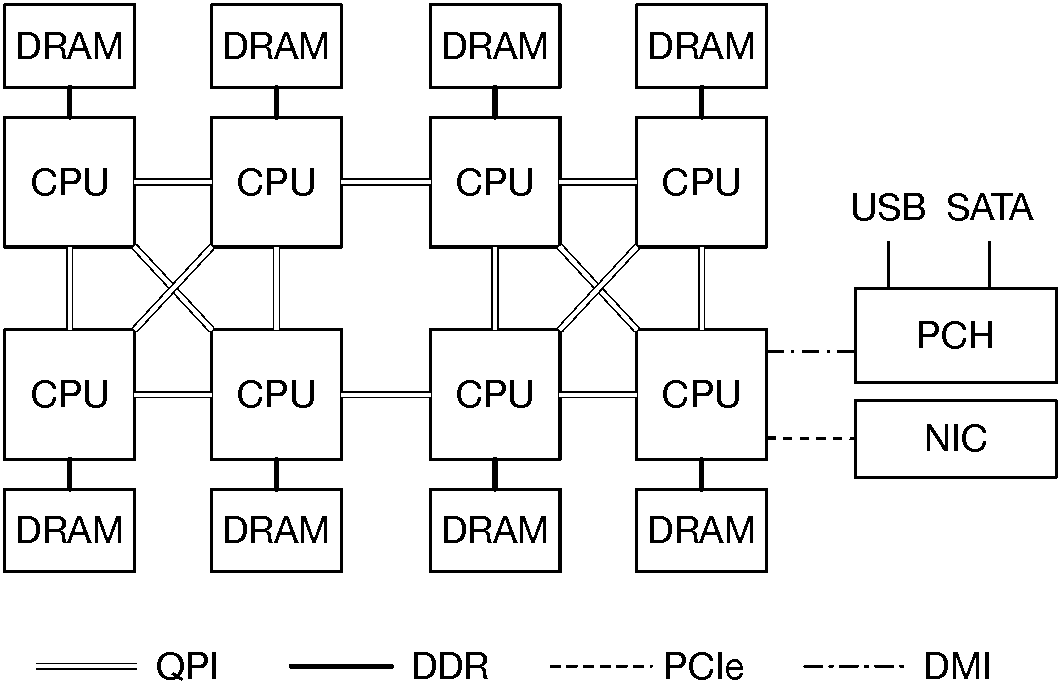
\includegraphics[width=85mm]{figures/motherboard.pdf}
  \caption{
    The motherboard structures that are most relevant to SGX.
  }
  \label{fig:motherboard}
\end{figure}

The CPU (described in \S~\ref{sec:cpu_die}) hosts the execution cores that run
the SMM, hypervisor, operating system, and application software. The computer's
main memory is provided by \textit{Dynamic Random-Access Memory} (DRAM) chips.

The \textit{Platform Controller Hub}~(PCH) houses (relatively) low-speed I/O
controllers driving the slower buses in the system, like SATA, used by storage
devices, and USB, used by input peripherals. In most systems, the PCH also
contains a service processor, called the Intel \textit{Management Engine}
(ME)~\cite{ruan2014intelme, ververis2010security}. The ME is intended for
remote system management and troubleshooting, and has tremendous privileges,
such as direct access to the network and to DRAM. These powers make the ME a
very high-value attack target (\S~\ref{sec:device_attacks}).

Motherboards also have a non-volatile (flash) memory chip that hosts firmware
which implements the \textit{Unified Extensible Firmware Interface}~(UEFI)
specification~\cite{forum2015uefi}. The firmware contains the boot code and the
code that executes in System Management Mode (SMM, \S~\ref{sec:rings}).

The components we care about are connected by the following buses: the
\textit{Quick-Path Interconnect}~(QPI~\cite{intel2009qpi}), a network of
point-to-point links that connect processors, the
\textit{double data rate}~(DDR) bus that connects a CPU to DRAM, the
\textit{Direct Media Interface}~(DMI) bus that connects a CPU to the PCH, the
\textit{Peripheral Component Interconnect Express}~(PCIe) bus that connects
a CPU to peripherals such as a \textit{Network Interface Card}~(NIC), and the
\textit {Serial Programming Interface}~(SPI) used by the PCH to communicate
with the flash memory.

The PCIe bus is an extended, point-to-point version of the PCI standard, which
provides a method for any peripheral connected to the bus to perform
\textit{Direct Memory Access}~(DMA), transferring data to and from DRAM without
involving an execution core and spending CPU cycles. The PCI standard includes
a configuration mechanism that assigns a range of DRAM to each peripheral, but
makes no provisions for preventing a rogue peripheral from accessing DRAM
outside the range that has been assigned to it.


\subsubsection{The Processor}
\label{sec:cpu_die}

An Intel processor's die, illustrated in Figure~\ref{fig:cpu_die}, is divided
into two broad areas: the \textit{core area} implements the instruction
execution pipeline typically associated with CPUs, while the \textit{uncore}
provides functions that were traditionally hosted on separate chips, but are
currently integrated on the CPU die to save power and improve latency.

\begin{figure}[hbt]
  \centering
  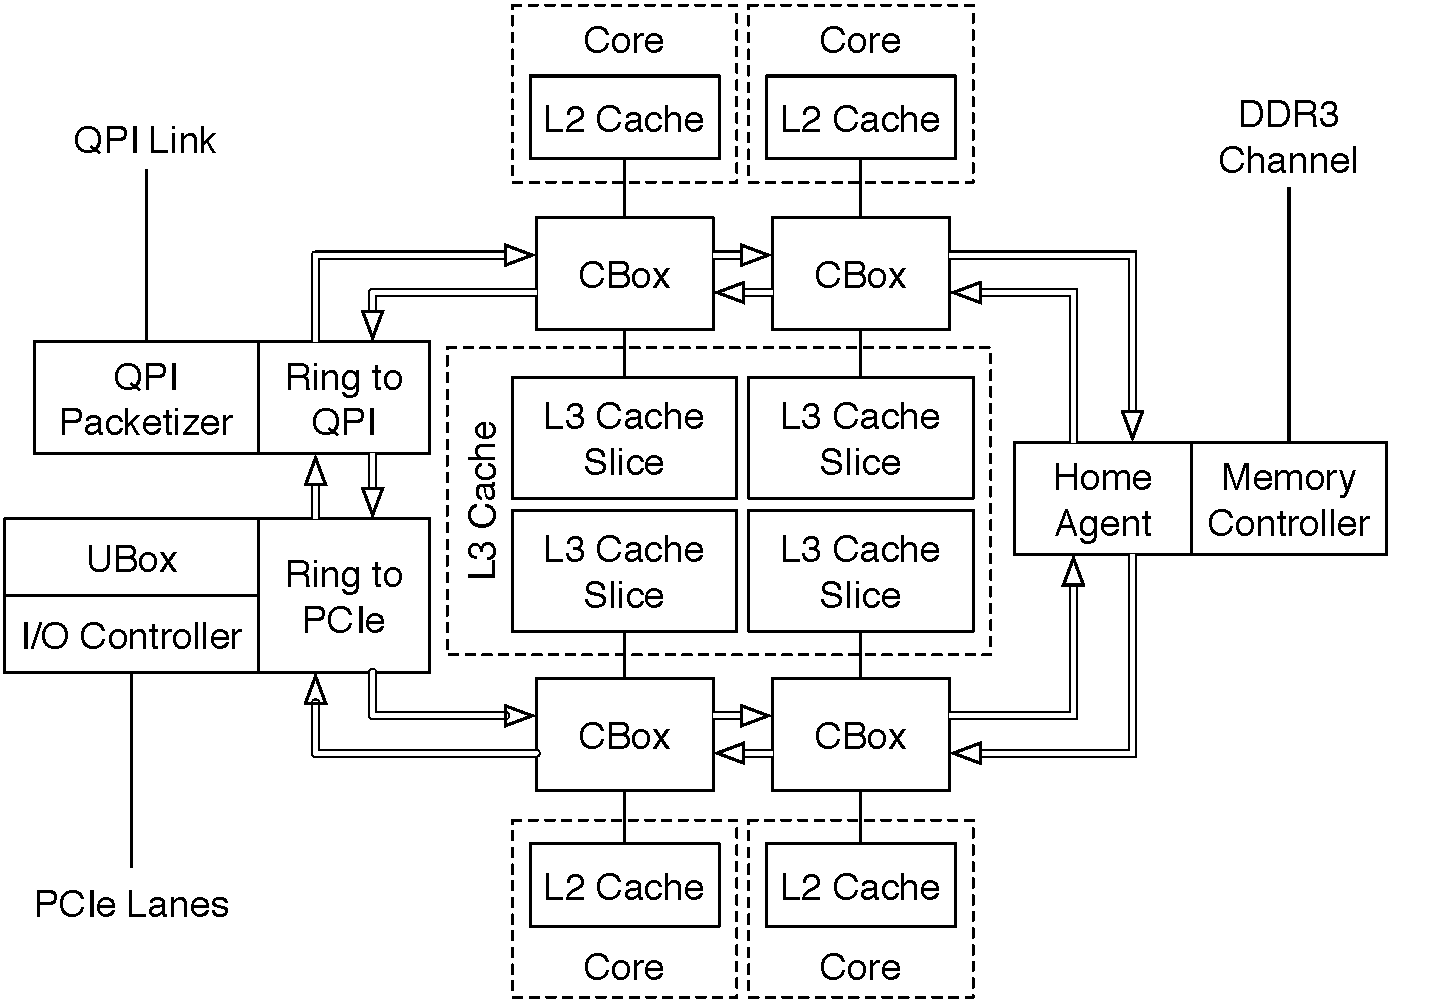
\includegraphics[width=85mm]{figures/cpu_die.pdf}
  \caption{
    The major components in a modern CPU package. \S~\ref{sec:cpu_die} gives
    an uncore overview. \S~\ref{sec:cpu_core} describes execution cores.
    \S~\ref{sec:cache_coherence} takes a deeper look at the uncore.
  }
  \label{fig:cpu_die}
\end{figure}

% Ring Interconnect and Last Level Cache: Optimization S 2.2.5.3
% System Agent: Optimization S 2.2.6

At a conceptual level, the uncore of modern processors includes an
\textit{integrated memory controller} (iMC) that interfaces with the DDR bus,
an \textit{integrated I/O controller} (IIO) that implements PCIe bus lanes and
interacts with the DMI bus, and a growing number of integrated peripherals,
such as a \textit{Graphics Processing Unit} (GPU). The uncore structure is
described in some processor family datasheets \cite{intel2014datasheet,
intel2010datasheet}, and in the overview sections in Intel's uncore performance
monitoring documentation \cite{intel2014uncore, intel2012uncore,
intel2010uncore}.

Security extensions to the Intel architecture, such as TXT and SGX, rely on the
fact that the processor die includes the memory and I/O controller, and thus
can prevent any device from accessing protected memory areas via
\textit{Direct Memory Access} (DMA) transfers. \S~\ref{sec:cache_coherence}
takes a deeper look at the uncore organization and at the machinery used to
prevent unauthorized DMA transfers.


\subsubsection{The Core}
\label{sec:cpu_core}

Virtually all modern Intel processors have core areas consisting of multiple
copies of the execution core circuitry, each of which is called a
\textit{core}.  At the time of this writing, desktop-class Intel CPUs have 4
cores, and server-class CPUs have as many as 18 cores.

Most Intel CPUs feature \textit{hyper-threading}, which means that a core
(shown in Figure~\ref{fig:cpu_core}) has two copies of the register files
backing the execution context described in \S~\ref{sec:registers}, and can
execute two separate streams of instructions simultaneously. Hyper-threading
increases the utilization of the shared fetch, decode and execution units, in
the presence of memory stalls.

\begin{figure}[hbt]
  \centering
  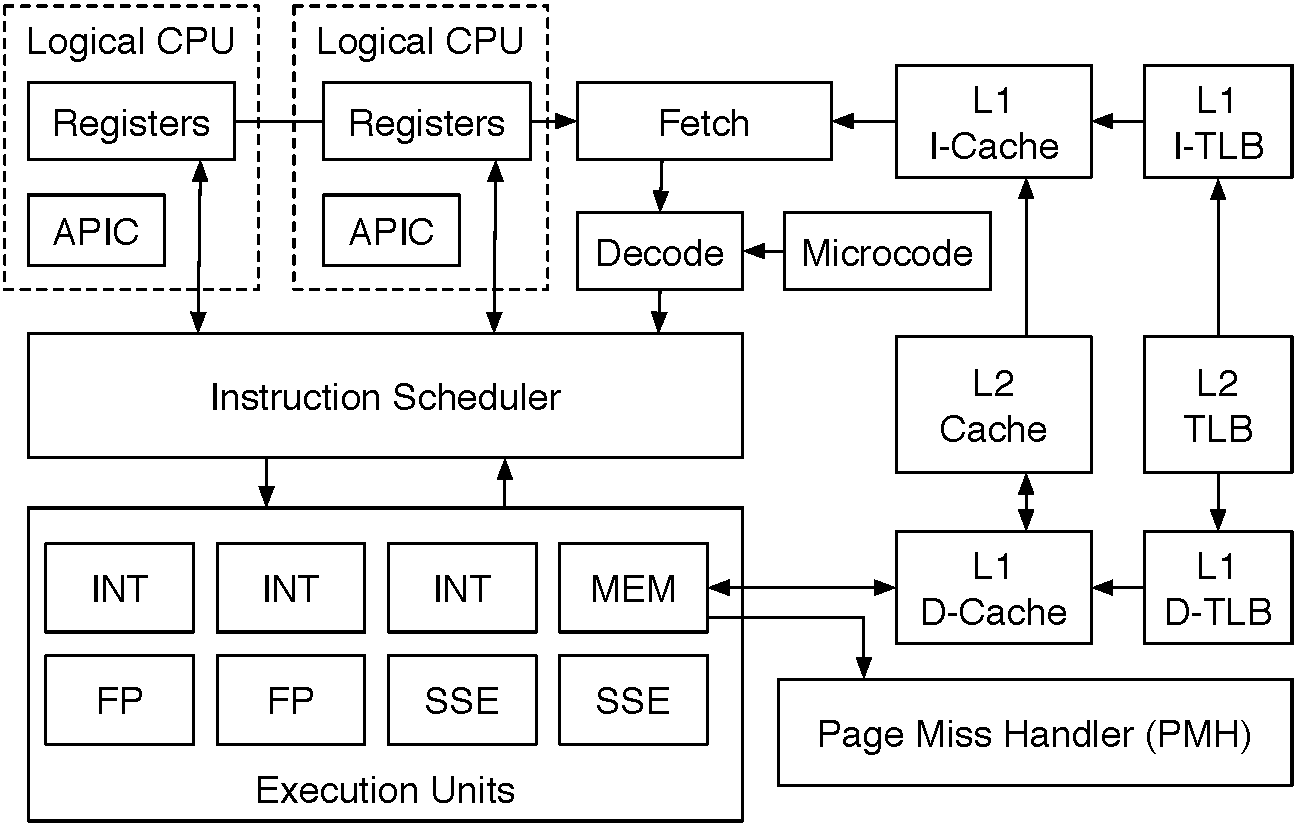
\includegraphics[width=85mm]{figures/cpu_core.pdf}
  \caption{
    CPU core with two logical processors. Each logical processor has its own
    execution context and LAPIC (\S~\ref{sec:interrupts}). All the other core
    resources are shared.
  }
  \label{fig:cpu_core}
\end{figure}

A hyper-threaded core is exposed to system software as two \textit{logical
processors}~(LPs), also named \textit{hardware threads} in the Intel
documentation. The logical processor abstraction allows the code used to
distribute work across processors in a multi-processor system to function
without any change on multi-core hyper-threaded processors.

The high level of resource sharing introduced by hyper-threading introduces a
security vulnerability. Software running on one logical processor can use the
high-resolution performance counter (\texttt{RDTSCP},
\S~\ref{sec:address_spaces}) \cite{petters1999making} to get information about
the instructions and memory access patterns of another piece of software that
is executed on the other logical processor on the same core.
